%!TEX root = ../main.tex

\subsection{Geometric component}
\label{ss:geometric_component}
Let us emphasize again that the only used information for the construction of the geometric and normal component are the three vertices with associated normals, that define a single primitive. The vertices contain the vertex \textit{xyz}-coordinates together with a unique shared normal per vertex, i.e., the normal of each vertex is the same for every primitive using that vertex. Figure \ref{fig:method:input_primitive} shows an illustration of an input primitive. Each point-normal triangle construction starts with an input primitive of this form.

\begin{figure}
	\centering
	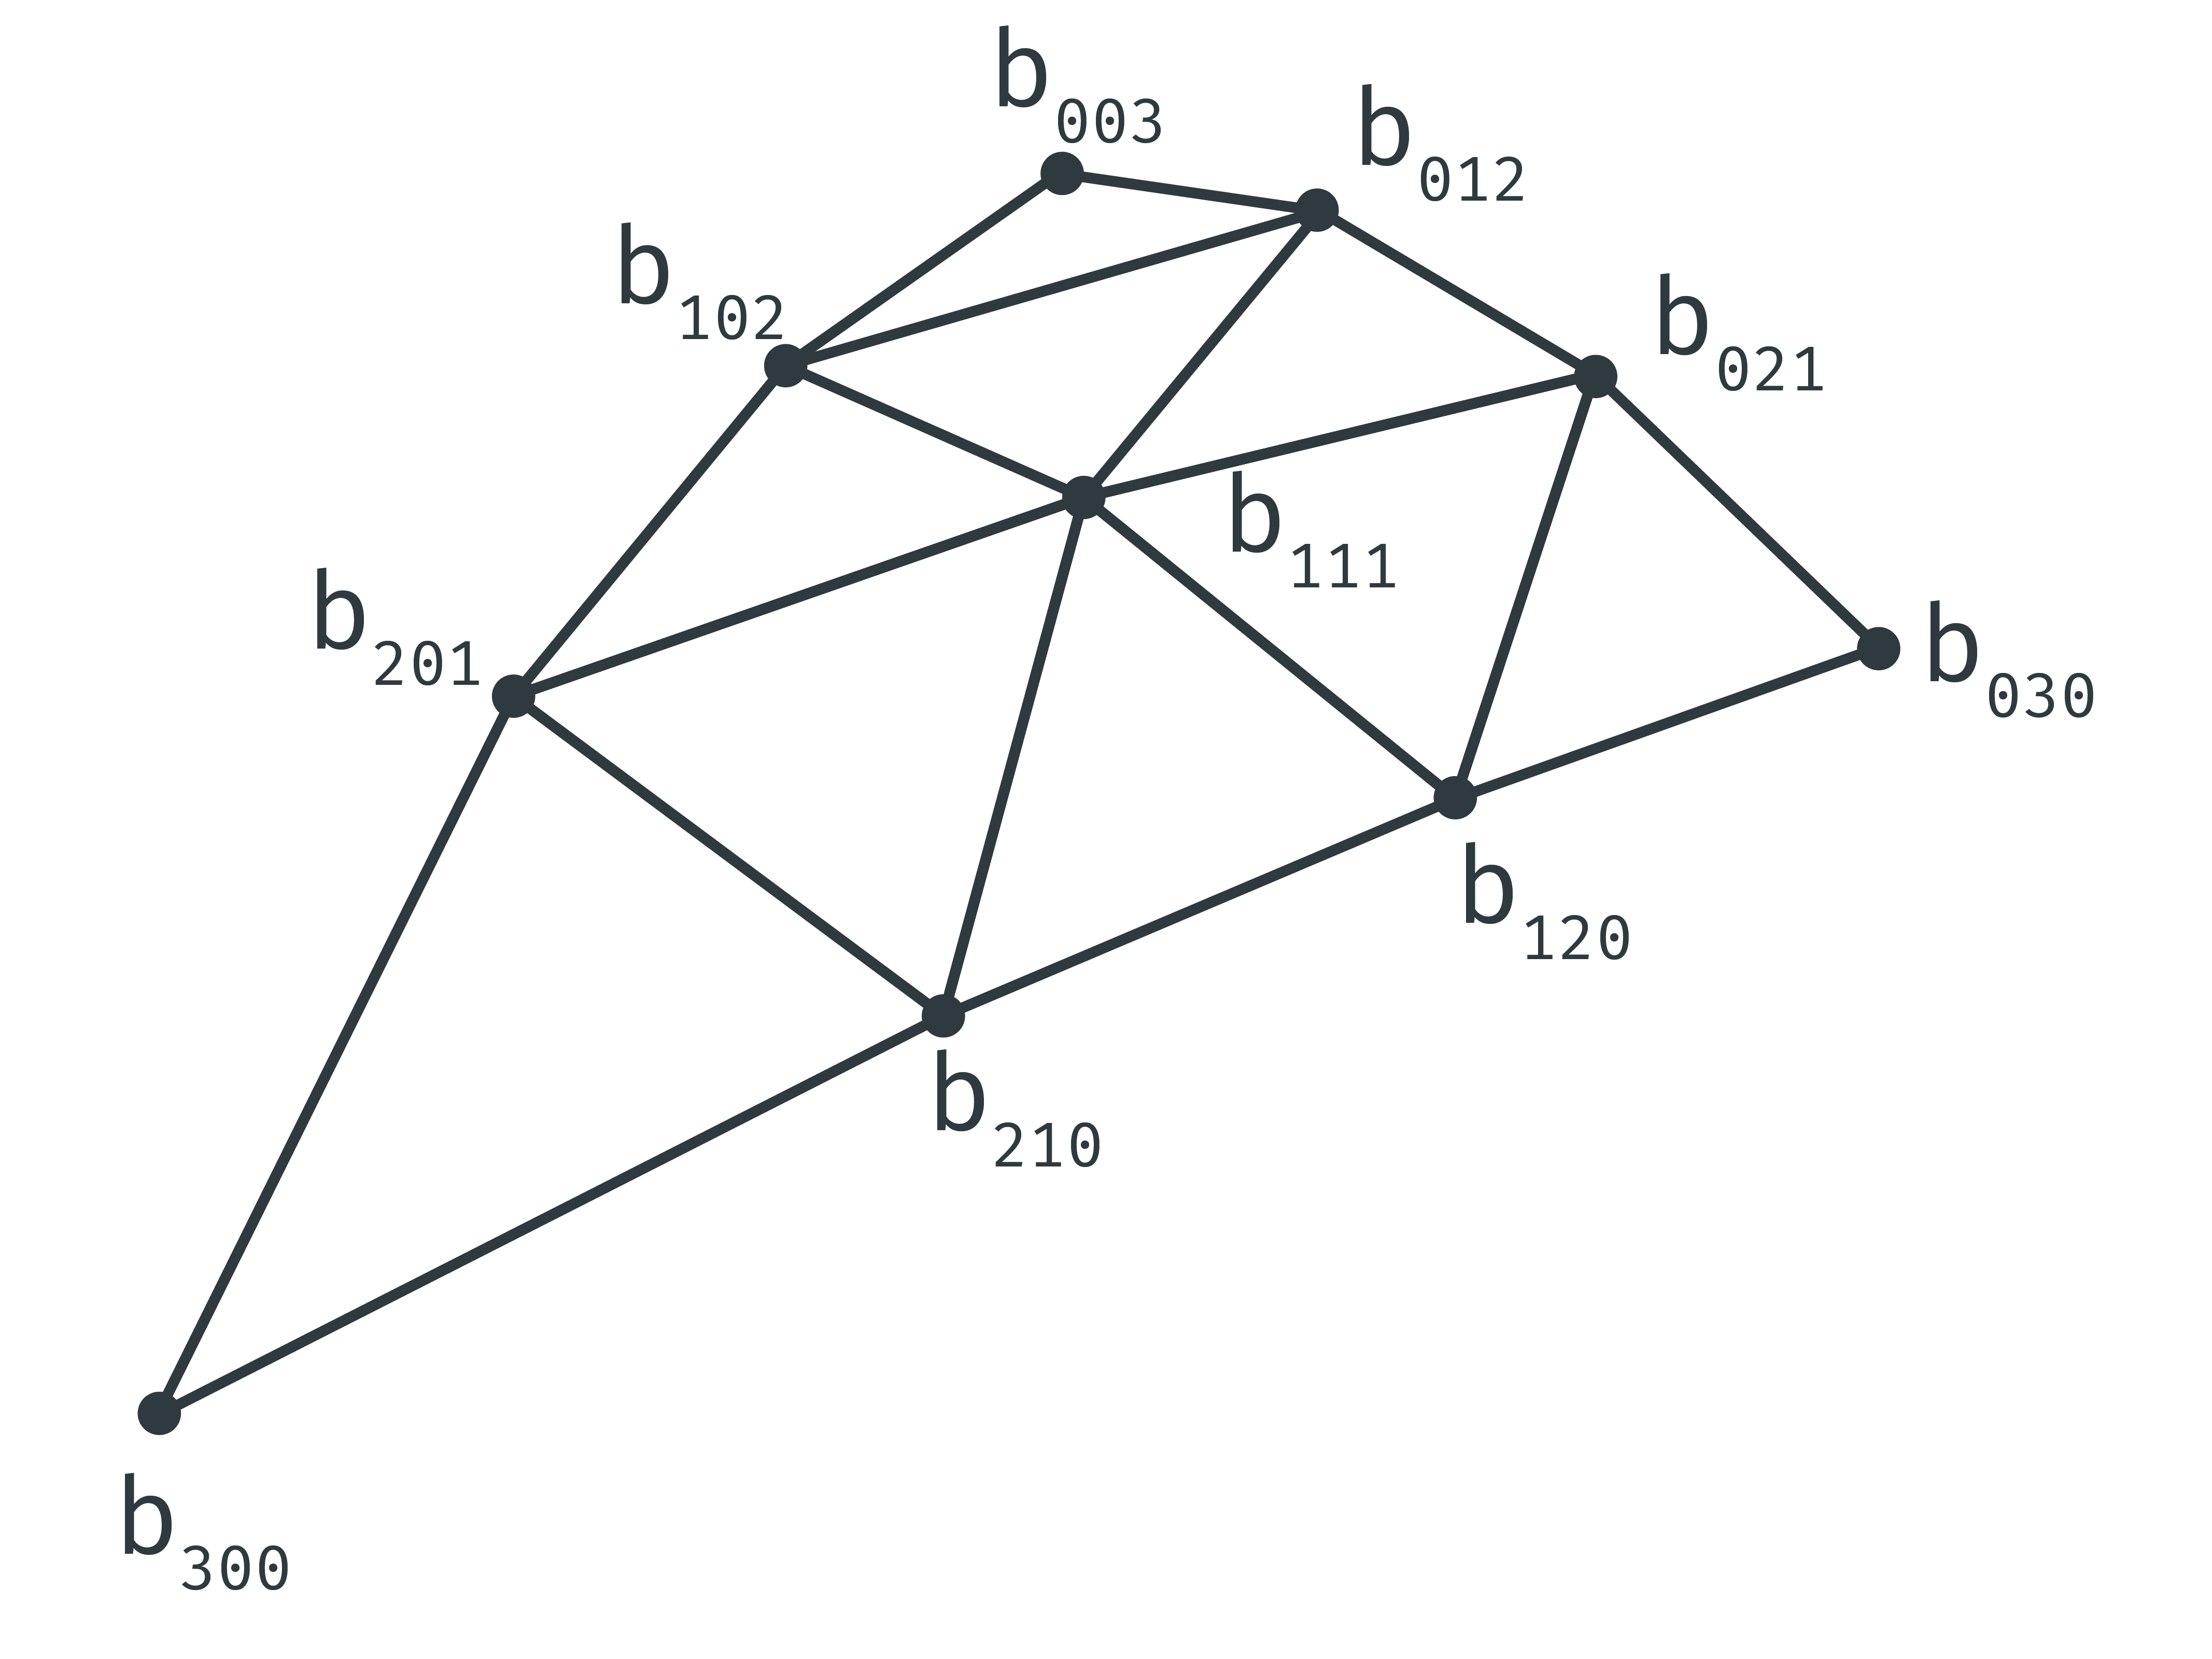
\includegraphics[width=0.45\textwidth]{./content/img/method/geometry.png}
	\caption{The geometric component of a point-normal triangle, i.e. the control net of a cubic Bézier triangle.}
	\label{fig:method:control_net}
\end{figure}
%
% ## Geometric component defined by triangluar cubic Bezier patch.
%
In the next subsection we discuss the definition of the geometry of a point-normal triangle. In subsection \crefs{sss:control_point_construction} we discuss the construction of the control points that define the geometry. 

\subsubsection{Basic form}
The geometric component of a point-normal triangle is defined as a triangular cubic Bézier patch. Such a patch $b(u,v)$ is defined as follows:
%
\begin{align}
\noalign{$b(u,v): \quad R^2 \mapsto R^3,\quad$ for $w = 1 - u - v, \quad u, v, w \geq 0$}
\begin{split}\label{eq:method:cubic_bezier_patch}
    b(u,v) ={}& \sum_{i + j + k = 3} b_{ijk}\frac{3!}{i!j!k!} u^i v^j w^k\\
      	   ={}& b_{300}w^3 + b_{030}u^3 + b_{003}v^3\\
      	    {}& + b_{210}3w^3 + b_{120}3wu^2 + b_{201}3w^2v\\
      	    {}& + b_{021}3u^2v + b_{102}2wv^2 + b_{012}3uv^2\\
      	    {}& + b_{111}6wuv.
\end{split}
\end{align}
%
The $b_{ijk}$ parameters in equation \ref{eq:method:cubic_bezier_patch} are the control points of the patch, also called coefficients. In \cref{fig:method:control_net} the visualization of the network of these control points is shown. We group the coefficients in three different groups, as their construction differs:
%
\begin{align*}
	\text{vertex coefficients: } {}&  b_{300},\ b_{030},\ b_{003} \\
	\text{tangent coefficients: } {}&  b_{210},\ b_{120},\ b_{021},\ b_{012},\ b_{102},\ b_{201}\\
	\text{center coefficient: }   {}&  b_{111}\\
\end{align*}

The formula in \eqref{eq:method:cubic_bezier_patch} can be used to evaluate any point parameterized by the barycentric coordinates $(u,v,w)$, on the patch. This is used in the sub-triangulation stage of the rendering process. In this stage the cubic Bézier surface is approximated by using a number of smaller flat triangles; these flat triangles are the triangles that are actually rendered. The number of sub-triangles is determined by the level of detail (lod). For the original sub-triangulation we refer the reader to \textcite{vlachos2001curved}, as this is where the implementation presented here deviates from the original. Details about this are provided in \crefs{s:implementation}.

As stated above the definition of the geometry of a point-normal triangle is a cubic Bézier patch. This degree of patches is a trade-off between simplicity, visual performance, and computational cost. Quadratic patches do not provide the same modeling range of a surface as a cubic patch, \citeauthor{boubekeur2008phong} \cite{boubekeur2008phong}. For example, a cubic representation is necessary to capture inflections implied by the triangle position and normal data. \citeauthor{vlachos2001curved} state that there is no additional data to suggest a higher degree is needed, and that therefore they settled on the form of $b(u,v)$ as presented in \crefe{eq:method:cubic_bezier_patch}.

\subsubsection{Coefficients} \label{sss:control_point_construction}
This section discusses how the `curved' control net geometry, (see \cref{fig:method:control_net}) is calculated from the flat input primitive shown in \cref{fig:method:input_primitive}. The input primitive provides the positions $P_1, P_2, P_3 \in \Real^3$ and normals $N_1, N_2, N_3 \in \Real^3$. The coefficients $b_{ijk}$ are computed as follows:
%
\begin{enumerate}[label=(\roman*)]
	\item 
		Initially, the coefficients $b_{ijk}$ are spread uniformly, i.e., the intermediate position of $b_{ijk}$ is calculated using the formula $(i P_i + j P_2 + kP_3) / 3$. 
	\item 
		The intermediate positions of the vertex coefficients are the same as their final positions, see equation \eqref{eq:method:vertex_coefficients}. Their intermediate position places them at the vertices of the input triangle, and this is where they are required to stay to keep the mesh watertight.
	\item 
		The tangent coefficients are placed at their final position by projecting the intermediate position into the tangent plane of the closest corner, see equation \eqref{eq:method:tangent_coefficients}. This is illustrated in \cref{fig:method:geometry_tangent_projection.png}.
	\item The center coefficient is moved to the average of the tangent coefficients plus $1/2$ times the distance it had to travel from its intermediate position, see equation \eqref{eq:method:center_coefficient}.
\end{enumerate}
%
\begin{figure}
	\centering
	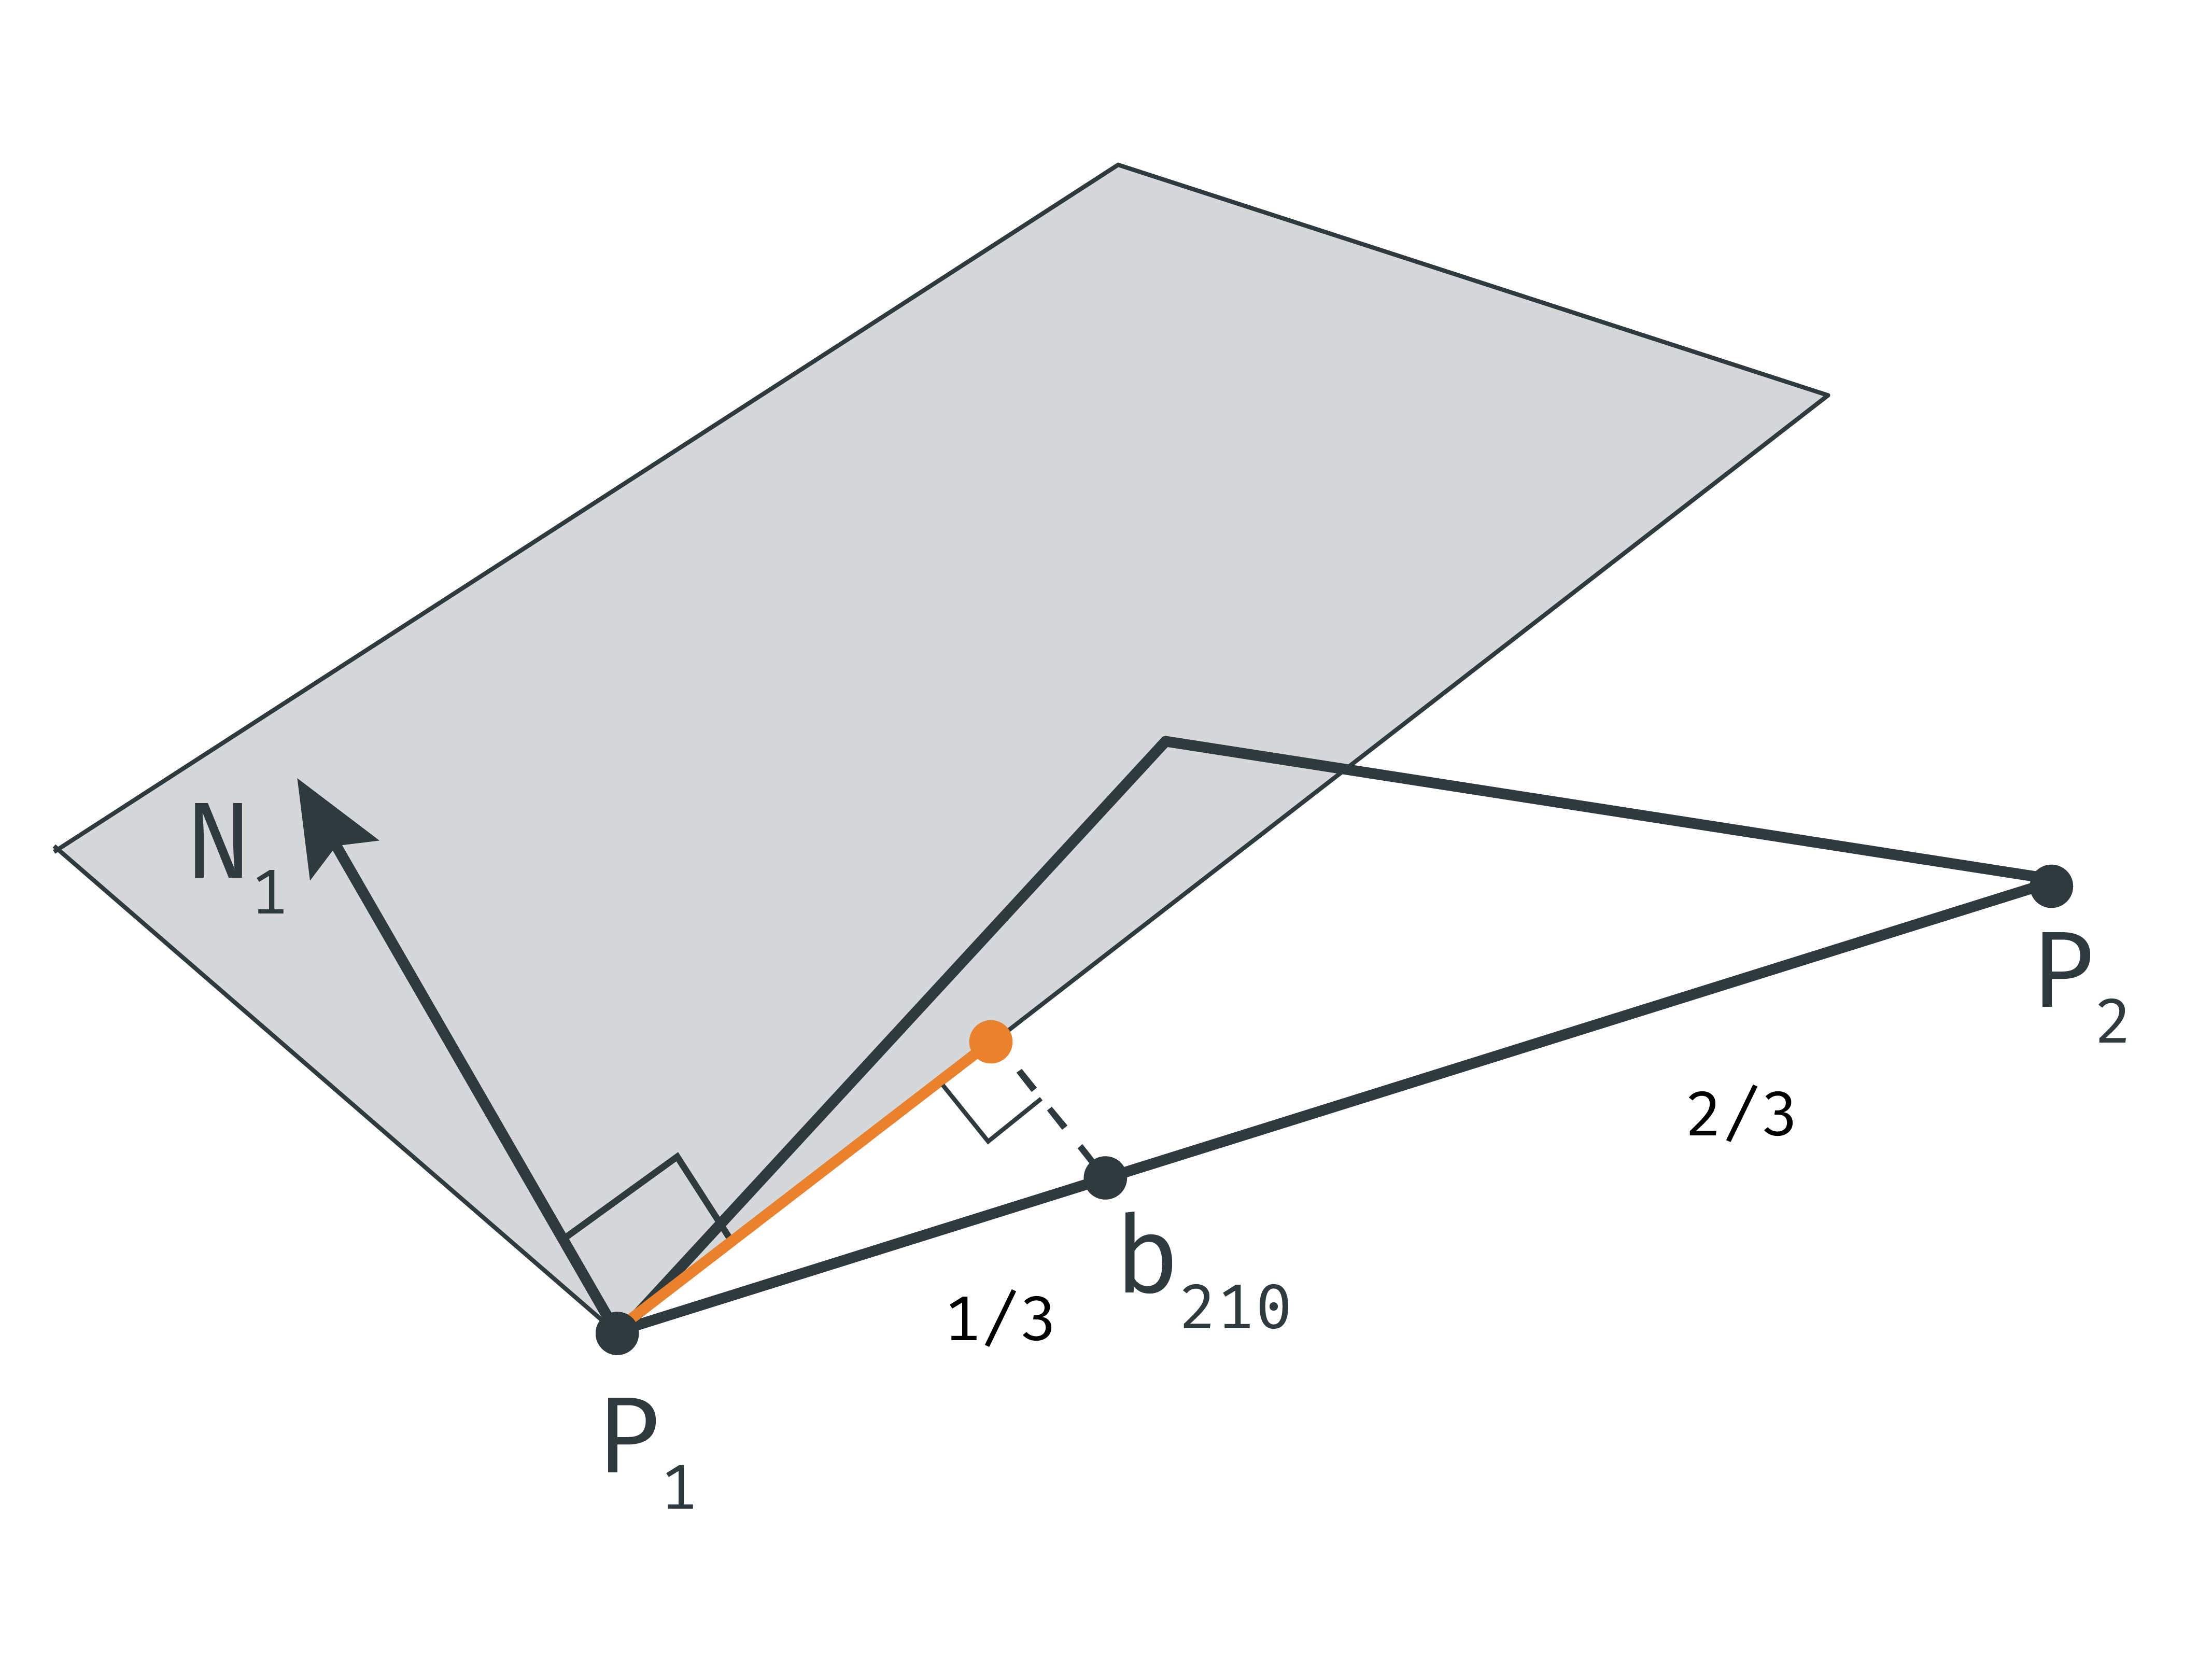
\includegraphics[width=0.45\textwidth]{./content/img/method/geometry_tangent_projection.png}
	\caption{Projection of a tangent coefficient $b_{210}$ to the tangent plane of the closes corner $P_1$.}
	\label{fig:method:geometry_tangent_projection.png}
\end{figure}


The following set of formulas describe how the positions of the coefficients are calculated. For clarity, we group together the formulas in the same way as the coefficients. This gives the following formulas for the \textit{vertex coefficients}:
\begin{align}\label{eq:method:vertex_coefficients}
	b_{300} = P_1,\ b_{030} = P_2,\ b_{003} = P_3.
\end{align}

The tangent coefficients are given by the projection of a point $Q$ onto the plane defined by the normal $N$ of the point $P$. The projected point $Q'$ is then given by: $Q' = Q - wN$, where $w = (Q - P) \cdot N$. Using this, the following set of formulas give the positions of the \textit{tangent coefficients}:
\begin{align}\label{eq:method:tangent_coefficients}
	w_{ij} = {}& (P_j - P_i) \cdot N_i \in \Real \nonumber\\
	b_{210} = {}& (2 P_1 + P_2 - w_{12}N_1) / 3,\nonumber\\
	b_{120} = {}& (2 P_2 + P_1 - w_{21}N_2) / 3,\nonumber\\
	b_{021} = {}& (2 P_2 + P_3 - w_{23}N_2) / 3, \\
	b_{012} = {}& (2 P_3 + P_2 - w_{32}N_3) / 3,\nonumber\\
	b_{102} = {}& (2 P_3 + P_1 - w_{31}N_3) / 3,\nonumber\\
	b_{201} = {}& (2 P_1 + P_3 - w_{13}N_1) / 3. \nonumber
\end{align}

The last coefficient is the center coefficient which is, as stated before, moved to the average of the previous computed tangent coefficients plus $1/2$ times the distance it traveled from its intermediate location to that average position. The \textit{center coefficient}, is computed by:
\begin{align}\label{eq:method:center_coefficient}
	E = {}& (b_{210} + b_{120} + b_{021} \nonumber \\
		{}& + b_{012} + b_{102} + b_{201}) / 6, \nonumber\\
	V = {}& (P_1 + P_2 + P_3) / 3, \\
	b_{111} = {}& E + (E - V) / 2. \nonumber
\end{align}
Combining \eqref{eq:method:vertex_coefficients} through \eqref{eq:method:center_coefficient} transforms the input primitive (see \cref{fig:method:input_primitive}) to the control net shown in \cref{fig:method:control_net}.

\subsubsection{Properties}
\label{sss:method:geometric:properties}
\citeauthor{vlachos2001curved} have shown that point-normal triangles do not deviate too much from the original triangle. This is an important property since this ensures that the shape of the model is preserved and adjacent triangles do not interfere with each other. 

By demanding shared normals, i.e., one unique normal per vertex, the boundary between two point-normal triangles is generated by the same algorithm, thus the surface is water tight. Except at the corners, PN triangles do not usually join with tangent continuity \cite{vlachos2001curved}. \Cref{fig:method:cracks} illustrates what happens if normals are not shared.

\begin{figure}
	\plaatje{Moeten dit plaatje eigenlijk maken met driehoeken.}
	\centering
	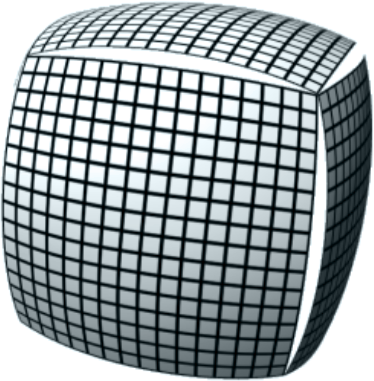
\includegraphics[width=0.45\textwidth]{./content/img/method/cracks.png}
	\caption{Illustration of what would happen if one renders a model using point-normal triangles where vertices have different normals, depending on the associated faces. Image taken from \cite{mcdonald2010crack}.}
	\label{fig:method:cracks}
\end{figure}